\documentclass[10pt,aspectratio=169]{beamer}

\usetheme{metropolis}
\metroset{progressbar=frametitle,numbering=fraction,block=fill,sectionpage=progressbar}

\usepackage{fontspec}
\usepackage{amsmath,amssymb,amsthm,mathtools,bbm}
\usepackage{booktabs}
\usepackage{tikz}
\usetikzlibrary{arrows.meta,positioning,calc,decorations.pathreplacing}
\usepackage{xcolor}

\definecolor{cktblue}{HTML}{1F4E79}
\definecolor{cktaccent}{HTML}{C0504D}
\definecolor{cktgray}{HTML}{595959}
\definecolor{cktgreen}{HTML}{2E7D32}
\setbeamercolor{frametitle}{bg=cktblue,fg=white}
\setbeamercolor{progress bar}{fg=cktaccent,bg=cktblue!20}
\setbeamercolor{title separator}{fg=cktaccent}
\setbeamercolor{alerted text}{fg=cktaccent}

\newcommand{\D}{D}
\newcommand{\mud}{\mu_{\underline{d}}}
\newcommand{\mudz}{\mu_{\underline{d}_0}}
\newcommand{\munb}{\mu_{\mathrm{unb}}}
\newcommand{\Deltad}{\Delta_{\underline{d}}}
\newcommand{\Deltadz}{\Delta_{\underline{d}_0}}
\newcommand{\Deltaunb}{\Delta_{\mathrm{unb}}}
\newcommand{\DS}{\mathcal{D}_{S}}
\newcommand{\dN}{d_{N}}
\newcommand{\dT}{d_{T}}

\title{Unbalanced individuals and the LCA restriction}
\subtitle{What we assume and what we could assume instead}
\date{\today}

\begin{document}

\begin{frame}[plain]
  \titlepage
\end{frame}

% ---------------------------------------------------------------
\begin{frame}{The problem: unbalanced individuals have no trajectory label}

  A trajectory $\underline d_i$ is a \textbf{full-wave} sequence of urban/rural status

  \vspace{0.6em}
  \begin{itemize}
    \item balanced individuals in IDN: observed in all 5 waves $\Rightarrow$ full trajectory
    \item unbalanced individuals: missing at least one wave $\Rightarrow$ no well-defined $\underline d_i$
  \end{itemize}

  \vspace{0.8em}
  Yet unbalanced individuals are 88--96\% of the sample

  \vspace{0.4em}
  Dropping them means dropping most of the data

\end{frame}

% ---------------------------------------------------------------
\begin{frame}{What we currently do: pool them into one extra cell}

  Think of it as a new cell alongside the balanced trajectory cells:

  \vspace{0.9em}
  \begin{center}
  \begin{tabular}{lcc}
    \toprule
     & \textbf{Rural consumption mean} & \textbf{Average urban return} \\
    \midrule
    Balanced cell $\underline d \in \mathcal D$ & $\mud$ & $\Deltad$ \\[0.2em]
    Pooled unbalanced cell & $\munb$ & $\Deltaunb$ \\
    \bottomrule
  \end{tabular}
  \end{center}

  \vspace{1em}
  In the regression, this is implemented by adding an unbalanced dummy $U_i$ \\
  and its interaction with the urban indicator $\D_{it}$

  \vspace{0.4em}
  Their coefficients \emph{are} $\munb$ and $\Deltaunb - \Deltadz$ --- just relabeled

\end{frame}

% ---------------------------------------------------------------
\begin{frame}{What LCA says about balanced cells}

  The LCA restriction (A5) at the individual level: $\Delta_i = \beta + \phi\, \theta_i$

  \vspace{0.8em}
  Averaged within a trajectory cell, this gives the \textbf{cell-level LCA}:
  \[
    \alert{\Deltad = \Deltadz + \phi\, (\mud - \mudz)} \qquad \text{for every } \underline d \in \DS
  \]

  \vspace{0.6em}
  Every balanced switcher cell has one free parameter ($\mud$)\\
  The return $\Deltad$ is determined by $\mud$ through LCA

  \vspace{0.8em}
  This is what lets us extrapolate returns to non-migrants ($\dN$, $\dT$) along the LCA line

\end{frame}

% ---------------------------------------------------------------
\begin{frame}{What we're \emph{not} imposing on the unbalanced cell}

  The pooled unbalanced cell, in our current spec, has \alert{two} free parameters:
  \[
    \munb \quad \text{and} \quad \Deltaunb
  \]

  They are estimated independently. Nothing in the current spec ties them together.

  \vspace{1em}
  \textbf{If LCA held on the unbalanced cell too}, they would satisfy
  \[
    \alert{\Deltaunb = \Deltadz + \phi\,(\munb - \mudz)}
  \]
  the same line that every switcher cell lies on

  \vspace{0.6em}
  We are not imposing this. We let the data fit $\Deltaunb$ freely.

\end{frame}

% ---------------------------------------------------------------
\begin{frame}{The LCA line, in a picture}

  \begin{center}
  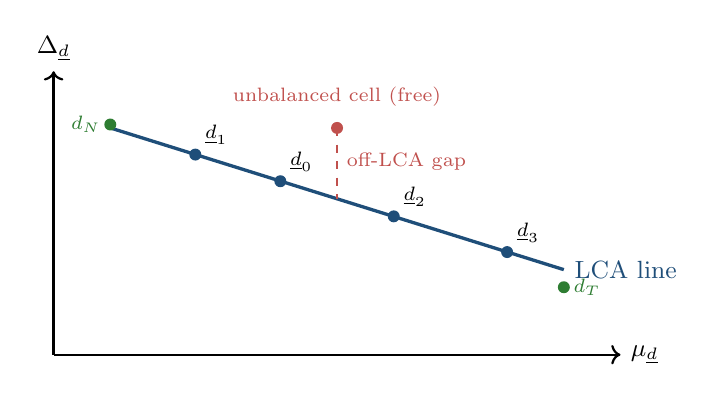
\begin{tikzpicture}[scale=0.72]
    \draw[->,thick] (0,0) -- (10,0) node[right] {\small $\mud$};
    \draw[->,thick] (0,0) -- (0,5) node[above] {\small $\Deltad$};

    \draw[cktblue,very thick] (1,4) -- (9,1.5) node[right,cktblue] {\small LCA line};

    \fill[cktblue] (2.5,3.53) circle (3pt) node[above right,black] {\scriptsize$\underline d_1$};
    \fill[cktblue] (4,3.06) circle (3pt) node[above right,black] {\scriptsize$\underline d_0$};
    \fill[cktblue] (6,2.44) circle (3pt) node[above right,black] {\scriptsize$\underline d_2$};
    \fill[cktblue] (8,1.81) circle (3pt) node[above right,black] {\scriptsize$\underline d_3$};

    \fill[cktgreen] (1,4.06) circle (3pt) node[left,cktgreen] {\scriptsize$\dN$};
    \fill[cktgreen] (9,1.19) circle (3pt) node[right,cktgreen] {\scriptsize$\dT$};

    \fill[cktaccent] (5,4) circle (3pt);
    \node[cktaccent,above] at (5,4.2) {\scriptsize unbalanced cell (free)};
    \draw[cktaccent,dashed,thick] (5,4) -- (5,2.75);
    \node[cktaccent,right] at (5,3.4) {\scriptsize off-LCA gap};
  \end{tikzpicture}
  \end{center}

  \vspace{0.2em}
  \footnotesize Balanced switchers $\underline d_0, \underline d_1, \ldots$ lie on the LCA line by construction. Non-migrants $\dN, \dT$ are extrapolated to the line. The unbalanced pooled cell sits wherever the data puts it --- potentially off the line.

\end{frame}

% ---------------------------------------------------------------
\begin{frame}{Option 1 (current): leave $\Deltaunb$ unconstrained}

  \begin{center}
    \begin{minipage}{0.85\textwidth}
    \textbf{Parameters for the unbalanced cell:} $\munb$ and $\Deltaunb$ (two free)\\[0.3em]
    \textbf{Moment conditions:} separate moments pin each one down\\[0.3em]
    \textbf{Interpretation:} we let the data fit the unbalanced-cell return without assuming LCA applies there
    \end{minipage}
  \end{center}

  \vspace{0.9em}
  \textbf{Pro.} Robust if LCA fails on the unbalanced cell (e.g., if attrition selects on $\theta_i$ in a way that breaks the LCA line)

  \vspace{0.5em}
  \textbf{Con.} Leaves information on the table. Unbalanced individuals don't help identify $\phi$.

  \vspace{0.5em}
  This is what's in the paper now

\end{frame}

% ---------------------------------------------------------------
\begin{frame}{Option 2 (cheap swap): impose LCA on the unbalanced cell}

  Replace the free return with the LCA-implied value:
  \[
    \Deltaunb \equiv \Deltadz + \phi\,(\munb - \mudz)
  \]

  \vspace{0.6em}
  Now only $\munb$ is a free parameter for the unbalanced cell

  The return $\Deltaunb$ is determined by $\munb$ and $\phi$, exactly as for every balanced switcher cell

  \vspace{1em}
  \textbf{What changed.} One fewer free parameter. The unbalanced cell becomes just another point on the LCA line, with mean $\munb$.

  \vspace{0.5em}
  \textbf{What's new.} Unbalanced individuals now contribute to identifying $\phi$ through the same LCA restriction as every switcher cell.

\end{frame}

% ---------------------------------------------------------------
\begin{frame}{Why this is cheap and principled}

  \textbf{Cheap}
  \begin{itemize}
    \item one constraint added to the GMM spec: $\Deltaunb = \Deltadz + \phi(\munb - \mudz)$
    \item no new dummies, no rewriting \texttt{handle\_trajectory\_groups}
    \item re-estimation on three countries, one afternoon
  \end{itemize}

  \vspace{0.8em}
  \textbf{Principled}
  \begin{itemize}
    \item LCA (A5) is assumed to hold at the individual level for \emph{everyone}
    \item if it holds for balanced individuals, it should hold for unbalanced individuals too --- why would a missing wave break a structural restriction?
    \item imposing LCA on the unbalanced cell is just being consistent with what we already claim
  \end{itemize}

\end{frame}

% ---------------------------------------------------------------
\begin{frame}{The restriction is testable}

  Under the current (free-$\Deltaunb$) specification, compute both sides:

  \vspace{0.8em}
  \begin{itemize}
    \item \textbf{Left side:} $\hat\Deltaunb$ from the GMM output
    \item \textbf{Right side:} $\hat\Deltadz + \hat\phi\,(\hat\munb - \hat\mudz)$ from the other GMM estimates
  \end{itemize}

  \vspace{0.8em}
  Three possible outcomes:

  \vspace{0.3em}
  \begin{itemize}
    \item \alert{they agree} $\Rightarrow$ LCA holds for unbalanced individuals; imposing it costs nothing
    \item \alert{they disagree slightly} $\Rightarrow$ LCA approximately holds; imposing it trades a bit of bias for precision
    \item \alert{they disagree a lot} $\Rightarrow$ interesting finding --- LCA fails on the unbalanced cell, suggesting attrition selects on comparative advantage
  \end{itemize}

  \vspace{0.6em}
  In all three cases, the check gives us information we don't currently have

\end{frame}

% ---------------------------------------------------------------
\begin{frame}{Why we didn't do this initially (speculation)}

  The current specification came from treating unbalanced individuals as a nuisance rather than as a cell:

  \vspace{0.8em}
  \begin{itemize}
    \item the goal was to keep them in the regression so that covariate coefficients $\gamma$ are estimated from the full sample
    \item their urban/rural differential was not the object of interest
    \item the unbalanced dummy and its urban interaction got added as ``controls,'' not as structural parameters
  \end{itemize}

  \vspace{0.8em}
  But treating the unbalanced group as a trajectory cell reveals:

  \vspace{0.3em}
  \begin{itemize}
    \item there is a well-defined $\munb$: the rural consumption mean in the unbalanced cell
    \item there is a well-defined $\Deltaunb$: its average urban return
    \item and the model already says these should be LCA-linked
  \end{itemize}

\end{frame}

% ---------------------------------------------------------------
\begin{frame}{Three options summarized}

  \begin{center}
  \footnotesize
  \begin{tabular}{p{2.9cm}p{3.1cm}p{3.1cm}p{3.3cm}}
    \toprule
     & \textbf{Option 1 (now)} & \textbf{Option 2} & \textbf{Option 3} \\
    \midrule
    Unbalanced cell & 1 pooled cell & 1 pooled cell & several cells by observed type \\[0.2em]
    Parameters & $\munb,\Deltaunb$ free & only $\munb$ free & $\munb^{(k)}$, each LCA-linked \\[0.2em]
    LCA imposed? & no & yes & yes \\[0.2em]
    Helps identify $\phi$? & no & yes, one cell & yes, several cells \\[0.2em]
    Effort & zero & half a day & one week \\
    \bottomrule
  \end{tabular}
  \end{center}

  \vspace{0.7em}
  \textbf{Recommendation:} Option 2 is the right next step. Cheap, structurally consistent with A5, and the testable-restriction check is informative either way. Option 3 only if Option 2 reveals something interesting.

\end{frame}

% ---------------------------------------------------------------
\begin{frame}{Takeaway}

  \begin{center}
    \begin{minipage}{0.9\textwidth}

    \textbf{The current approach treats the unbalanced pooled cell as exempt from LCA.}

    \vspace{0.8em}
    Its rural consumption mean $\munb$ and its average urban return $\Deltaunb$ are estimated as two independent free parameters.

    \vspace{0.8em}
    \textbf{Imposing LCA on the unbalanced cell means:} replacing the free return with the LCA-implied return $\Deltaunb = \Deltadz + \phi(\munb - \mudz)$.

    \vspace{0.8em}
    \textbf{Cost:} one constraint in the GMM spec.\\
    \textbf{Benefit:} one more cell contributing to $\hat\phi$, one less free parameter, internal consistency with A5, and a new testable restriction as diagnostic.

    \end{minipage}
  \end{center}

\end{frame}

\end{document}
